\documentclass[handout]{beamer}
\usepackage{array}
\usepackage{german}
\usepackage{graphicx}
\usepackage[utf8]{inputenc}
\usepackage[T1]{fontenc}
\usepackage{tikz}
\usepackage{qrcode}
\mode<beamer>{%
\usetheme{Copenhagen}
}
\usepackage[orientation=landscape,size=a3,debug,scale=2.7]{beamerposter}
\title[]{}
\begin{document}
\begin{frame}
\frametitle{%\hspace{0pt plus 1 filll}
MathSem 2021: Matrizen}
%\bigskip
\begin{columns}[t,onlytextwidth]
\begin{column}{0.32\textwidth}
%{%\bf
%\large Das Buch zum Seminar}
%\bigskip
%\vskip 1cm
\begin{center}
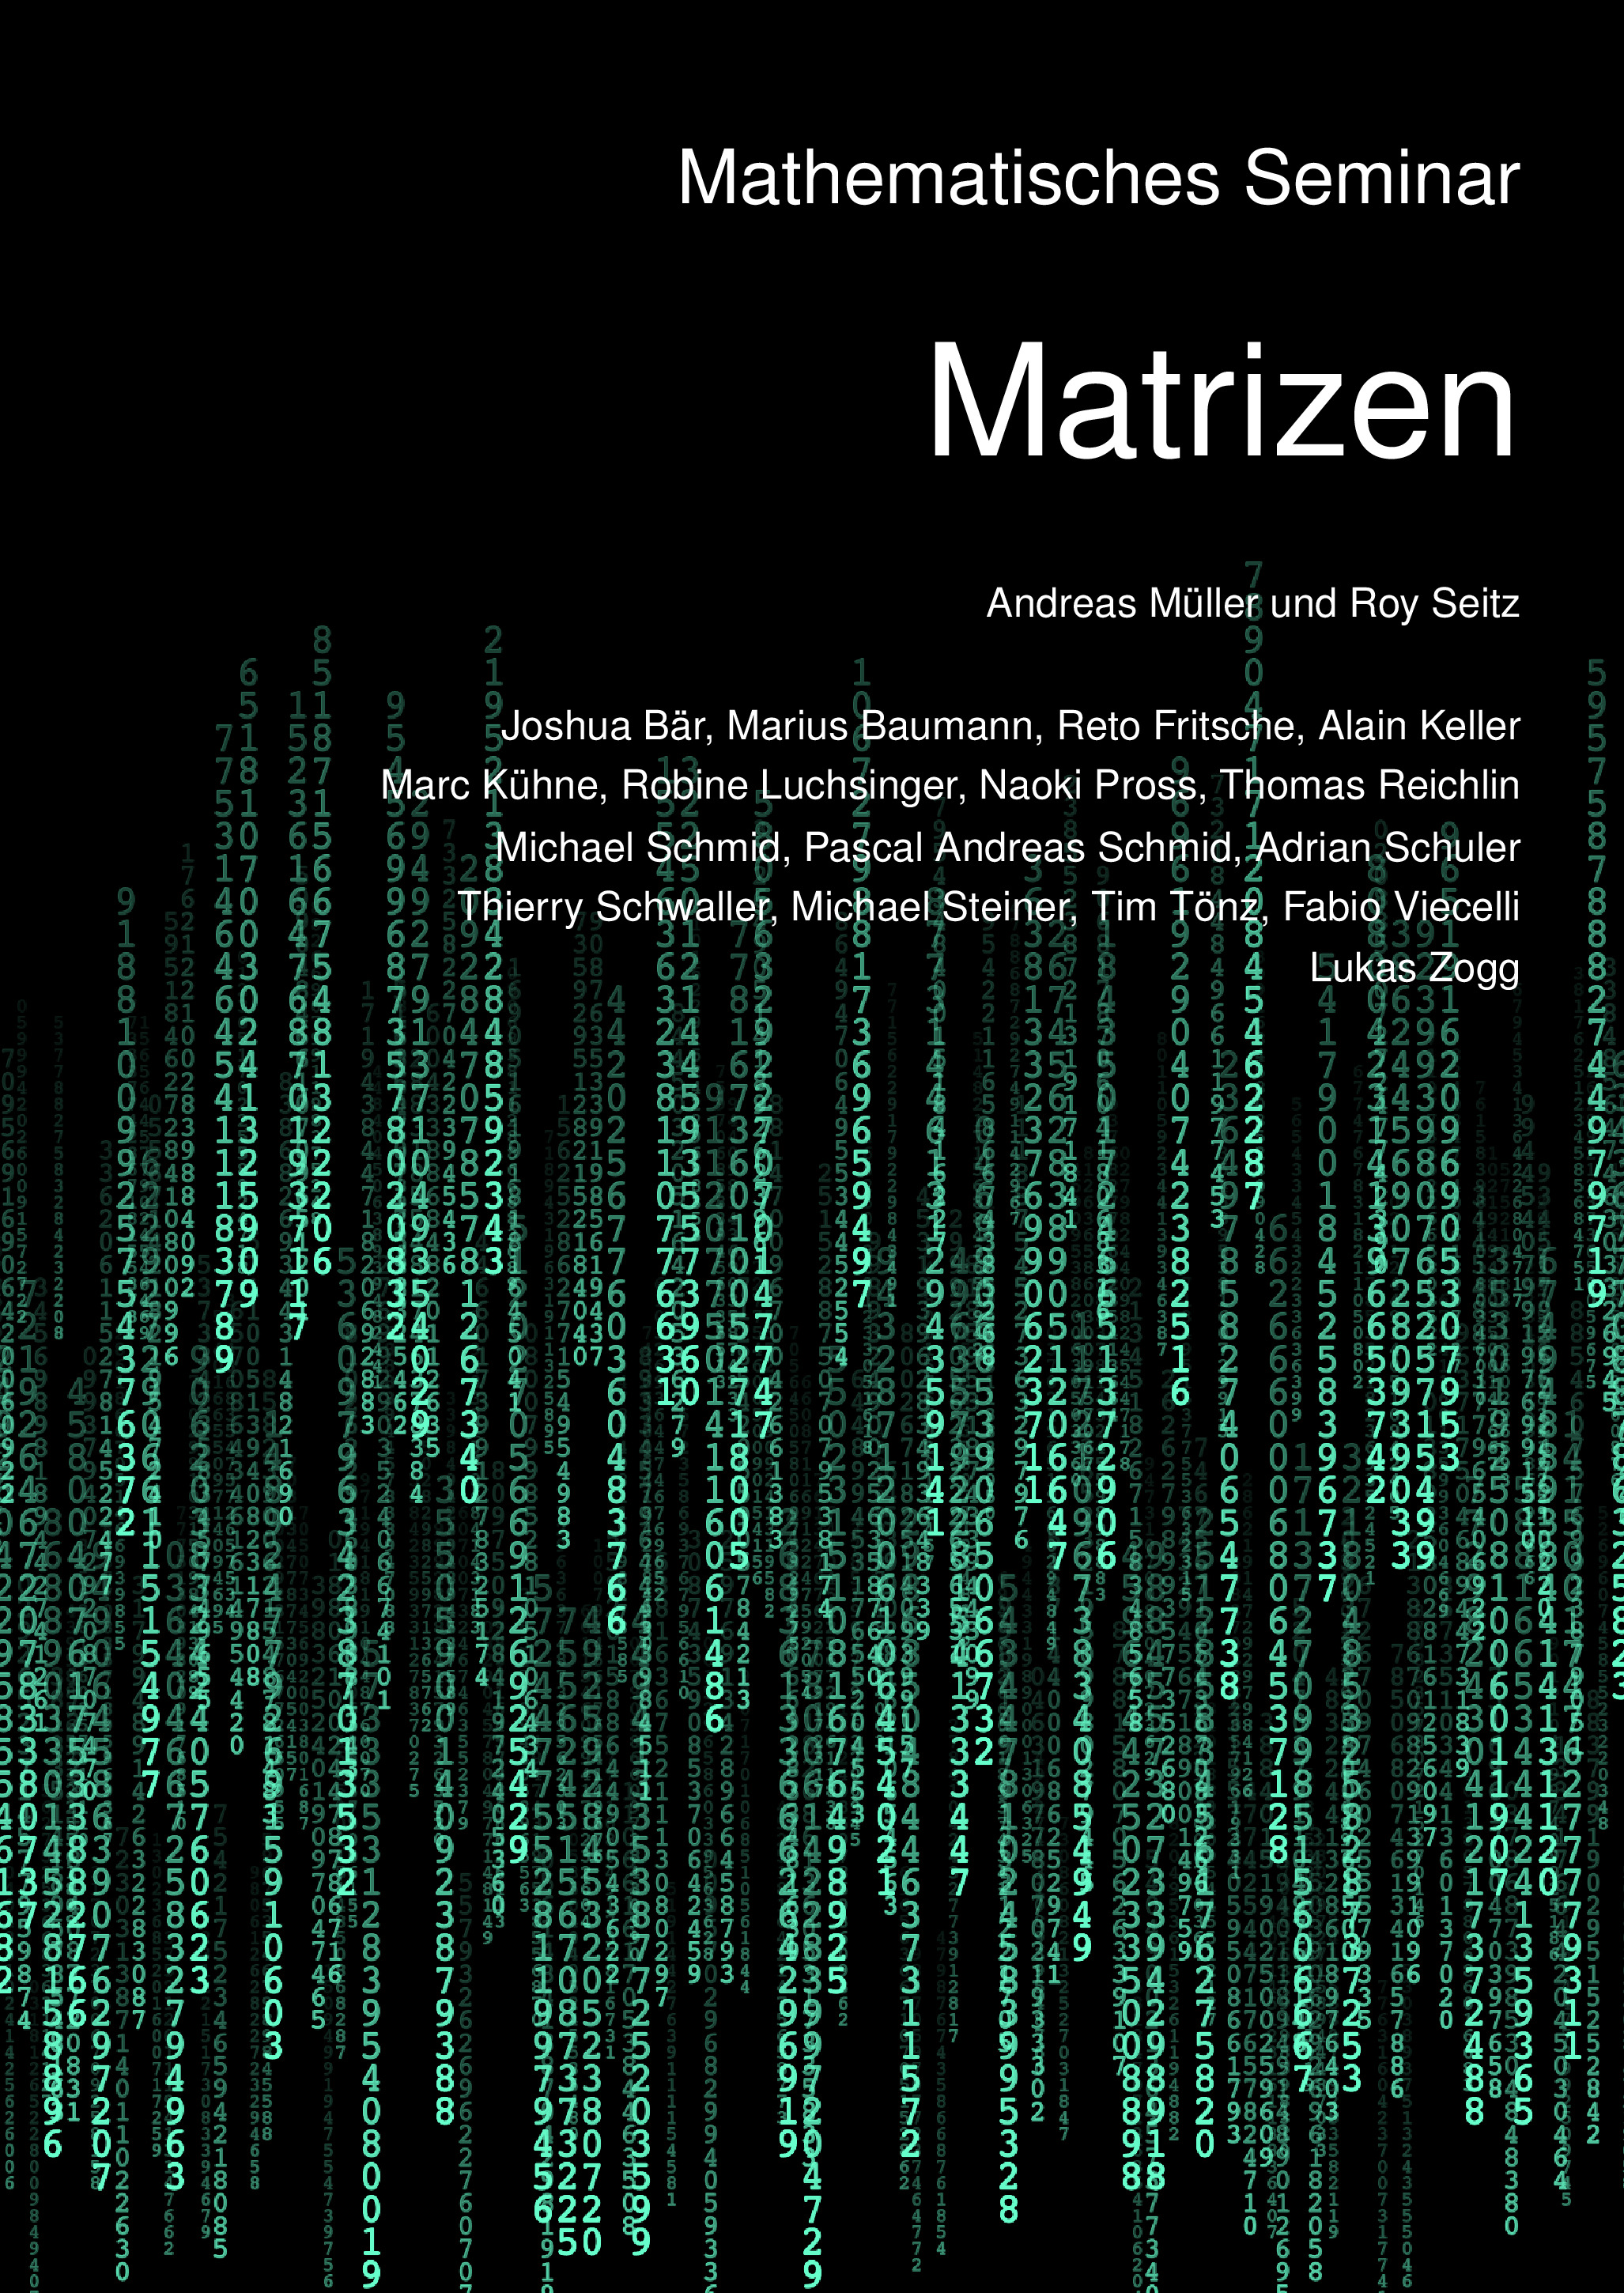
\includegraphics[width=\hsize]{../cover/buchcover.png}
\end{center}
\vskip 0.2cm
\bigskip
\bigskip
Erschienen im Herbst 2021.\\
Anfragen~an~Prof.~Dr.~Andreas~Müller,\\
{\texttt{andreas.mueller@ost.ch}}
\bigskip
\bigskip
\bigskip
%\vskip 1.2cm
\end{column}
\begin{column}{0.65\textwidth}
\begin{description}
\item[Teil 1:] Grundlagen
\begin{enumerate}
\item Zahlen
\item Vektoren und Matrizen
\item Polynome
\item Endliche Körper
\item Eigenwerte und Eigenvektoren
\item Permutationen
\item Matrizengruppen
\item Graphen
\item Wahrscheinlichkeitsmatrizen
\item Anwendungen in der Kryptographie
\item Kettenkomplexe und Homologie
\end{enumerate}
\item[Teil 2:] Anwendungen und weiterführende Themen
\begin{enumerate}
\setcounter{enumi}{11}
\item Robine Luchsinger und Pascal Andreas Schmid: {\em Verkehrsfluss und Verkehrsnetze}
\item Michael Schmid: {\em Schnelle Matrixmultiplikation}
\item Naoki Pross und Tim Tönz: {\em Crystal Math}
\item Joshua Bär und Michael Steiner: {\em Reed-Solomon-Code}
\item Alain Keller: {\em Iterierte Funktionsschemata}
\item Reto Fritsche: {\em McEliece-Kryptosystem}
\item Marius Baumann und Thierry Schwaller: {\em Geometrische Algebra}
\item Thomas Reichlin und Adrian Schuler: {\em Dreidimensionaler Spannungszustand}
\item Fabio Viecelli und Lukas Zogg: {\em Erdbebenmessung}
\item Marc Kühne: {\em Das Zuordnungsproblem und der Munkres-Algorithmus}
\end{enumerate}
\end{description}
\end{column}
\begin{column}{0.01\textwidth}
\llap{%
%\hbox to3cm{%
%\begin{center}
%\begin{tikzpicture}[>=latex,thick]
%\node at (0,0) {
%\qrcode[height=3cm]{https://github.com/AndreasFMueller/SeminarMatrizen/releases/download/v1.0.0/SeminarMatrizen.pdf}
%};
%\node at (0,0) {

\includegraphics[width=10mm]{../cover/mathman.png}
%};
%\end{tikzpicture}
%\end{center}
%}%
}
\end{column}
\end{columns}
\end{frame}
\end{document}
